
\textbf{Column 1: -}

\begin{quote}
It is the only column that is guaranteed to have no other additional
non-zero elements.
\end{quote}



\begin{minipage}[t]{\linewidth}\raggedright
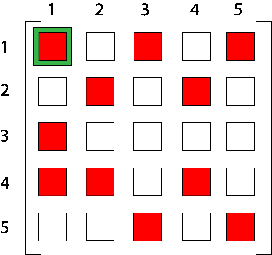
\includegraphics[width=1.2375in,height=1.16016in]{./Scheduler/media/image19.png}

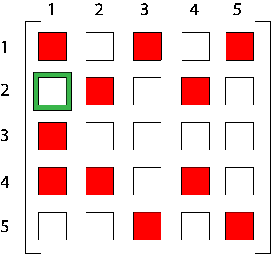
\includegraphics[width=1.23194in,height=1.15466in]{./Scheduler/media/image20.png}

\begin{quote}
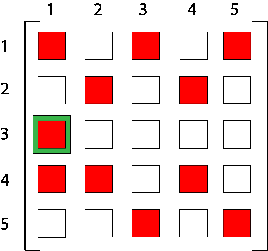
\includegraphics[width=1.21944in,height=1.14209in]{./Scheduler/media/image21.png}

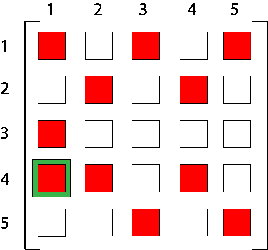
\includegraphics[width=1.21667in,height=1.13495in]{./Scheduler/media/image22.png}
\end{quote}
\end{minipage} \& \begin{minipage}[t]{\linewidth}\raggedright
\begin{quote}
According to equation 3.2a,\\
U1,1 = A1,1

According to equation 3.2a,\\
L2,1 = A2,1/U1,1 = 0\\
Since A2,1 is 0, the entire L2,1 equation will be neglected.

According to equation 3.2b,\\
L3,1 = A3,1/U1,1\\
~\\
~\\
~\\
According to equation 3.2b,\\
L4,1 = A4,1/U1,1
\end{quote}
\end{minipage} \\
\bottomrule
\end{longtable}

11

\begin{longtable}[]{@{}
  >{\raggedright\arraybackslash}p{(\columnwidth - 4\tabcolsep) * \real{0.33}}
  >{\raggedright\arraybackslash}p{(\columnwidth - 4\tabcolsep) * \real{0.33}}
  >{\raggedright\arraybackslash}p{(\columnwidth - 4\tabcolsep) * \real{0.33}}@{}}
\toprule
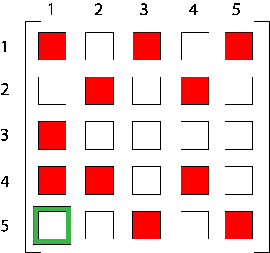
\includegraphics[width=1.22639in,height=1.14917in]{./Scheduler/media/image23.png}
& & \begin{minipage}[b]{\linewidth}\raggedright
\begin{quote}
According to equation 3.2b,\\
L5,1 = A5,1/U1,1 = 0\\
Since A5,1 is 0, the entire L5,1 equation will be neglected.
\end{quote}
\end{minipage} \\
\midrule

& & \\
& & \\
\textbf{Column 2: -} & & \\
\bottomrule
\end{longtable}

\begin{quote}
Column 2 onwards, there can be additional non-zero locations and MAC
operations will also come into play from here on.
\end{quote}



\begin{minipage}[t]{\linewidth}\raggedright
\begin{quote}
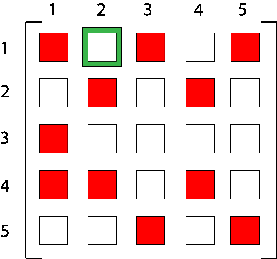
\includegraphics[width=1.25972in,height=1.17786in]{./Scheduler/media/image24.png}

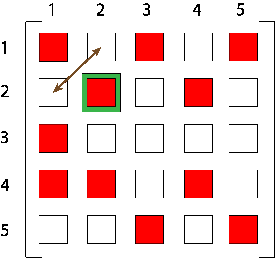
\includegraphics[width=1.25in,height=1.17273in]{./Scheduler/media/image25.png}

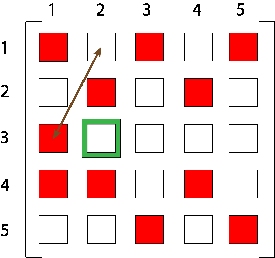
\includegraphics[width=1.25in,height=1.17273in]{./Scheduler/media/image26.png}

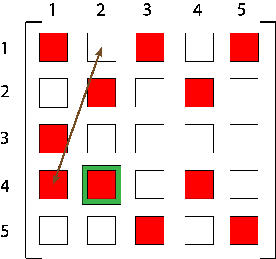
\includegraphics[width=1.25417in,height=1.17692in]{./Scheduler/media/image27.png}

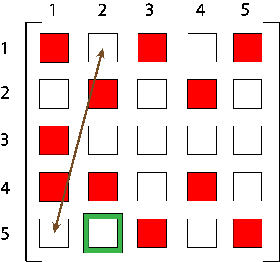
\includegraphics[width=1.27222in,height=1.19044in]{./Scheduler/media/image28.png}
\end{quote}
\end{minipage} & \begin{minipage}[t]{\linewidth}\raggedright
\begin{quote}
According to equation 3.2a,

U1,2 = A1,2 = 0

Since A1,2 is 0, U1,2 will be neglected.

According to equation 3.2a,

U2,2 = A2,2 -- L2,1*U1,2 = A2,2

Since both L2,1 \& U1,2 terms are 0, the multiplication operation can be
neglected.

According to equation 3.2b,

L3,2 = (A3,2 -- L3,1*U1,2)/U2,2 = 0\\
Since A3,2 \& U1,2 are 0, the entire L3,2 equation is neglected.

According to equation 3.2b,

L4,2 = (A4,2 -- L4,1*U1,2)/U2,2 = A4,2/U2,2\\
Since U1,2 is 0, the multiplication operation can be neglected.

According to equation 3.2b,

L5,2 = (A5,2 -- L5,1*U1,2)/U2,2 = 0\\
Since A5,2 \& U1,2 are 0, the entire L5,2 equation is neglected.
\end{quote}
\end{minipage} \\
\bottomrule
\end{longtable}

12

\textbf{Column 3: -}



\begin{minipage}[t]{\linewidth}\raggedright
\begin{quote}
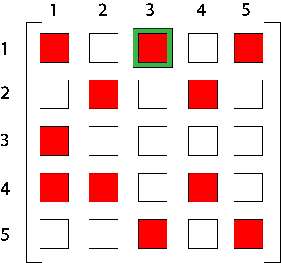
\includegraphics[width=1.275in,height=1.19333in]{./Scheduler/media/image29.png}

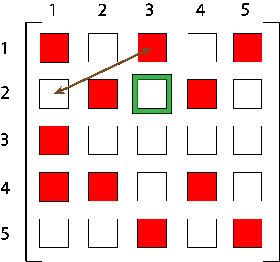
\includegraphics[width=1.27222in,height=1.19044in]{./Scheduler/media/image30.png}
\end{quote}

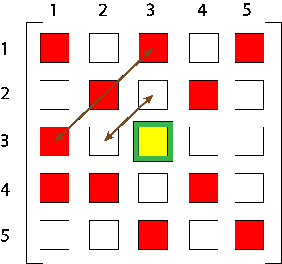
\includegraphics[width=1.28055in,height=1.19882in]{./Scheduler/media/image31.png}

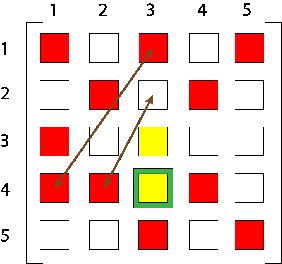
\includegraphics[width=1.28055in,height=1.19882in]{./Scheduler/media/image32.png}

\begin{quote}
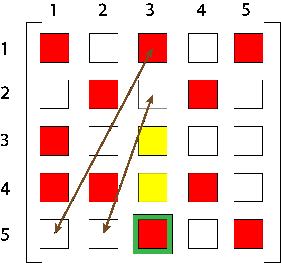
\includegraphics[width=1.275in,height=1.19333in]{./Scheduler/media/image33.png}
\end{quote}
\end{minipage} & \begin{minipage}[t]{\linewidth}\raggedright
\begin{quote}
According to equation 3.2a,

U1,3 = A1,3

According to equation 3.2a,

U2,3 = A2,3 -- L2,1*U1,3 = 0

Since A2,3 \& L2,1 = 0, the entire U2,3 equation can be neglected.

According to equation 3.2a,

U3,3 = A3,3 -- L3,1*U1,3 -- L3,2*U2,3 = -- L3,1*U1,3

Since both L3,2 \& U2,3 are zero, the second multiplication operation is neglected.
\end{quote}

Also, note that this is the first element in the fill-in-matrix that
converted from

\begin{quote}
zero to non-zero element. Hence marked with yellow color.

According to equation 3.2b,

L4,3 = (A4,3 -- L4,1*U1,3 -- L4,2*U2,3)/U3,3 = (-- L4,1*U1,3)/U3,3

Since U2,3 is zero, the second multiplication operation is neglected.
\end{quote}

Note that this element in the fill-in-matrix is converted to a non-zero
element.

\begin{quote}
Hence marked with yellow color.

According to equation 3.2b,

L5,3 = (A5,3 -- L5,1*U1,3 -- L5,2*U2,3)/U3,3 = A5,3/U3,3

Since L5,1 is 0, the 1st multiplication operation is neglected. Since
both L5,2 \& U2,3

are zeros, the second multiplication operation is also neglected.
\end{quote}
\end{minipage} \\
\bottomrule
\end{longtable}

\textbf{Column 4: -}

\begin{longtable}[]{@{}
  >{\raggedright\arraybackslash}p{(\columnwidth - 4\tabcolsep) * \real{0.33}}
  >{\raggedright\arraybackslash}p{(\columnwidth - 4\tabcolsep) * \real{0.33}}
  >{\raggedright\arraybackslash}p{(\columnwidth - 4\tabcolsep) * \real{0.33}}@{}}
\toprule
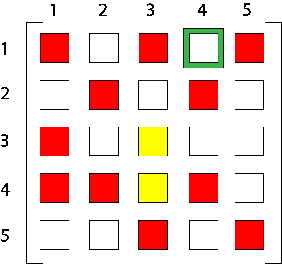
\includegraphics[width=1.28055in,height=1.19882in]{./Scheduler/media/image34.png}
& & \begin{minipage}[b]{\linewidth}\raggedright
\begin{quote}
According to equation 3.2a,
\end{quote}
\end{minipage} \\
\midrule

& & \begin{minipage}[t]{\linewidth}\raggedright
\begin{quote}
U1,4 = A1,4 = 0
\end{quote}
\end{minipage} \\
& & \begin{minipage}[t]{\linewidth}\raggedright
\begin{quote}
Since A1,4 is 0, U1,4 will be neglected.
\end{quote}
\end{minipage} \\
\begin{minipage}[t]{\linewidth}\raggedright
\begin{quote}
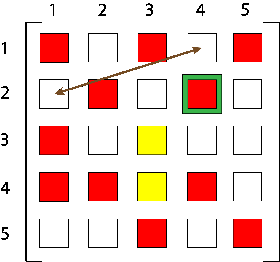
\includegraphics[width=1.27222in,height=1.19044in]{./Scheduler/media/image35.png}
\end{quote}
\end{minipage} & & \begin{minipage}[t]{\linewidth}\raggedright
\begin{quote}
According to equation 3.2a,
\end{quote}
\end{minipage} \\
& & \begin{minipage}[t]{\linewidth}\raggedright
\begin{quote}
U2,4 = A2,4 -- L2,1*U1,4 = A2,4
\end{quote}
\end{minipage} \\
& & \begin{minipage}[t]{\linewidth}\raggedright
\begin{quote}
Since both L2,1 \& U1,4 is 0, the multiplication term can be neglected.
\end{quote}
\end{minipage} \\
& & \\
\bottomrule
\end{longtable}

13



\begin{minipage}[t]{\linewidth}\raggedright
\begin{quote}
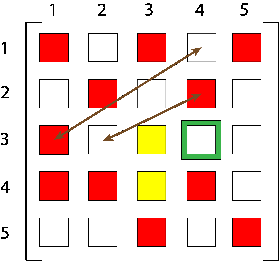
\includegraphics[width=1.26806in,height=1.18625in]{./Scheduler/media/image36.png}

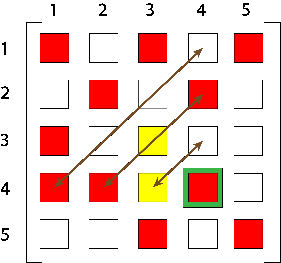
\includegraphics[width=1.275in,height=1.19333in]{./Scheduler/media/image37.png}

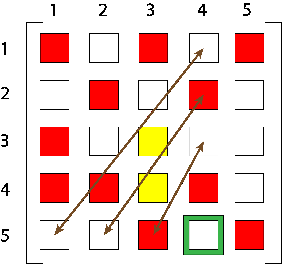
\includegraphics[width=1.28055in,height=1.19882in]{./Scheduler/media/image38.png}
\end{quote}
\end{minipage} & \begin{minipage}[t]{\linewidth}\raggedright
\begin{quote}
According to equation 3.2a,

U3,4 = A3,4 -- L3,1*U1,4 -- L3,2*U2,4 = 0

Since A3,4, U1,4 \& L3,2 are zeros, and the entire U3,4 equation can be
neglected.

According to equation 3.2a,

U4,4 = A4,4 -- L4,1*U1,4 -- L4,2*U2,4 -- L4,3*U3,4 = A4,4 -- L4,2*U2,4

Since U1,4 is 0, the 1st multiplication term is neglected, and since U3,4
is 0, the 3rd

The multiplication term is neglected.

According to equation 3.2b,

L5,4 = (A5,4 -- L5,1*U1,4 -- L5,2*U2,4 -- L5,3*U3,4)/U4,4 = 0

Sine A5,4 is 0, and one or both the operands is 0 for all the three
multiplication

terms, the entire L5,4 equation is neglected.
\end{quote}
\end{minipage} \\
\bottomrule
\end{longtable}

\textbf{Column 5: -}



\begin{minipage}[t]{\linewidth}\raggedright
\begin{quote}
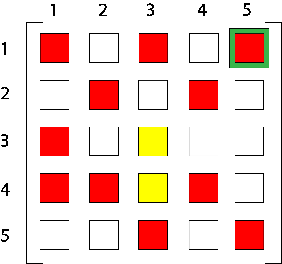
\includegraphics[width=1.28194in,height=1.20012in]{./Scheduler/media/image39.png}

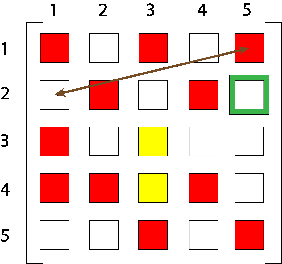
\includegraphics[width=1.28194in,height=1.20012in]{./Scheduler/media/image40.png}

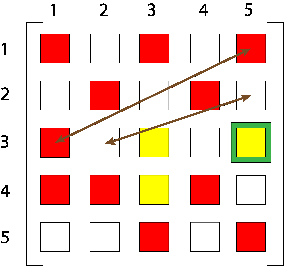
\includegraphics[width=1.29167in,height=1.2098in]{./Scheduler/media/image41.png}

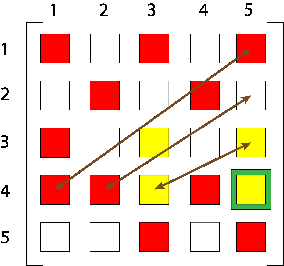
\includegraphics[width=1.29167in,height=1.2098in]{./Scheduler/media/image42.png}
\end{quote}
\end{minipage} & \begin{minipage}[t]{\linewidth}\raggedright
\begin{quote}
According to equation 3.2a,

U1,5 = A1,5

According to equation 3.2a,

U2,5 = A2,5 -- L2,1*U1,5 = 0

According to equation 3.2a,

U3,5 = A3,5 -- L3,1*U1,5 -- L3,2*U2,5 = -- L3,1*U1,5

According to equation 3.2a,

U4,5 = A4,5 -- L4,1*U1,5 -- L4,2*U2,5 -- L4,3*U3,5 = -- L4,1*U1,5 --
L4,3*U3,5
\end{quote}
\end{minipage} \\
\bottomrule
\end{longtable}

\begin{quote}
14
\end{quote}



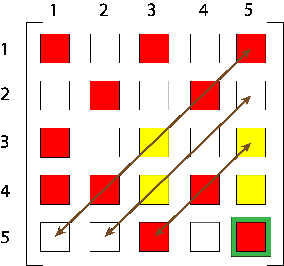
\includegraphics[width=1.29167in,height=1.2098in]{./Scheduler/media/image43.png}
& \begin{minipage}[t]{\linewidth}\raggedright
\begin{quote}
According to equation 3.2a,

U5,5 = A5,5 -- L5,1*U1,5 -- L5,2*U2,5 -- L5,3*U3,5 = A5,5 -- L5,3*U3,5
\end{quote}
\end{minipage} \\
\bottomrule
\end{longtable}

Now compare all the equations before and after symbolic analysis: -

\begin{longtable}[]{@{}
  >{\raggedright\arraybackslash}p{(\columnwidth - 12\tabcolsep) * \real{0.14}}
  >{\raggedright\arraybackslash}p{(\columnwidth - 12\tabcolsep) * \real{0.14}}
  >{\raggedright\arraybackslash}p{(\columnwidth - 12\tabcolsep) * \real{0.14}}
  >{\raggedright\arraybackslash}p{(\columnwidth - 12\tabcolsep) * \real{0.14}}
  >{\raggedright\arraybackslash}p{(\columnwidth - 12\tabcolsep) * \real{0.14}}
  >{\raggedright\arraybackslash}p{(\columnwidth - 12\tabcolsep) * \real{0.14}}
  >{\raggedright\arraybackslash}p{(\columnwidth - 12\tabcolsep) * \real{0.14}}@{}}
\toprule
\textbf{Col.}

\textbf{No.} & \begin{minipage}[b]{\linewidth}\raggedright
\begin{quote}
\textbf{Equations before symbolic analysis}
\end{quote}
\end{minipage} & \begin{minipage}[b]{\linewidth}\raggedright
\begin{quote}
\textbf{MAC}

\textbf{ops}
\end{quote}
\end{minipage} & \textbf{DIV}

\textbf{ops} & \textbf{Equations after}

\textbf{symbolic analysis} & \textbf{MAC}

\textbf{ops} & \begin{minipage}[b]{\linewidth}\raggedright
\begin{quote}
\textbf{DIV}

\textbf{ops}
\end{quote}
\end{minipage} \\
\midrule

1 & \begin{minipage}[t]{\linewidth}\raggedright
\begin{quote}
U1,1 = A1,1
\end{quote}
\end{minipage} & 0 & 0 & \begin{minipage}[t]{\linewidth}\raggedright
\begin{quote}
U1,1 = A1,1
\end{quote}
\end{minipage} & 0 & 0 \\
& \begin{minipage}[t]{\linewidth}\raggedright
\begin{quote}
L2,1 = A2,1/U1,1
\end{quote}
\end{minipage} & 0 & 1 & \begin{minipage}[t]{\linewidth}\raggedright
\begin{quote}
-
\end{quote}
\end{minipage} & 0 & 0 \\
& \begin{minipage}[t]{\linewidth}\raggedright
\begin{quote}
L3,1 = A3,1/U1,1
\end{quote}
\end{minipage} & 0 & 1 & \begin{minipage}[t]{\linewidth}\raggedright
\begin{quote}
L3,1 = A3,1/U1,1
\end{quote}
\end{minipage} & 0 & 1 \\
& \begin{minipage}[t]{\linewidth}\raggedright
\begin{quote}
L4,1 = A4,1/U1,1
\end{quote}
\end{minipage} & 0 & 1 & \begin{minipage}[t]{\linewidth}\raggedright
\begin{quote}
L4,1 = A4,1/U1,1
\end{quote}
\end{minipage} & 0 & 1 \\
& \begin{minipage}[t]{\linewidth}\raggedright
\begin{quote}
L5,1 = A5,1/U1,1
\end{quote}
\end{minipage} & 0 & 1 & \begin{minipage}[t]{\linewidth}\raggedright
\begin{quote}
-
\end{quote}
\end{minipage} & 0 & 0 \\
2 & \begin{minipage}[t]{\linewidth}\raggedright
\begin{quote}
U1,2 = A1,2
\end{quote}
\end{minipage} & 0 & 0 & \begin{minipage}[t]{\linewidth}\raggedright
\begin{quote}
-
\end{quote}
\end{minipage} & 0 & 0 \\
& \begin{minipage}[t]{\linewidth}\raggedright
\begin{quote}
U2,2 = A2,2 -- L2,1*U1,2
\end{quote}
\end{minipage} & 1 & 0 & \begin{minipage}[t]{\linewidth}\raggedright
\begin{quote}
U2,2 = A2,2
\end{quote}
\end{minipage} & 0 & 0 \\
& \begin{minipage}[t]{\linewidth}\raggedright
\begin{quote}
L3,2 = (A3,2 -- L3,1*U1,2)/U2,2
\end{quote}
\end{minipage} & 1 & 1 & \begin{minipage}[t]{\linewidth}\raggedright
\begin{quote}
-
\end{quote}
\end{minipage} & 0 & 0 \\
& \begin{minipage}[t]{\linewidth}\raggedright
\begin{quote}
L4,2 = (A4,2 -- L4,1*U1,2)/U2,2
\end{quote}
\end{minipage} & 1 & 1 & \begin{minipage}[t]{\linewidth}\raggedright
\begin{quote}
L4,2 = A4,2/U2,2
\end{quote}
\end{minipage} & 0 & 1 \\
& \begin{minipage}[t]{\linewidth}\raggedright
\begin{quote}
L5,2 = (A5,2 -- L5,1*U1,2)/U2,2
\end{quote}
\end{minipage} & 1 & 1 & \begin{minipage}[t]{\linewidth}\raggedright
\begin{quote}
-
\end{quote}
\end{minipage} & 0 & 0 \\
3 & \begin{minipage}[t]{\linewidth}\raggedright
\begin{quote}
U1,3 = A1,3
\end{quote}
\end{minipage} & 0 & 0 & \begin{minipage}[t]{\linewidth}\raggedright
\begin{quote}
U1,3 = A1,3
\end{quote}
\end{minipage} & 0 & 0 \\
& \begin{minipage}[t]{\linewidth}\raggedright
\begin{quote}
U2,3 = A2,3 -- L2,1*U1,3
\end{quote}
\end{minipage} & 1 & 0 & \begin{minipage}[t]{\linewidth}\raggedright
\begin{quote}
-
\end{quote}
\end{minipage} & 0 & 0 \\
& \begin{minipage}[t]{\linewidth}\raggedright
\begin{quote}
U3,3 = A3,3 -- L3,1*U1,3 -- L3,2*U2,3
\end{quote}
\end{minipage} & 2 & 0 & \begin{minipage}[t]{\linewidth}\raggedright
\begin{quote}
U3,3 = -- L3,1*U1,3
\end{quote}
\end{minipage} & 1 & 0 \\
& \begin{minipage}[t]{\linewidth}\raggedright
\begin{quote}
L4,3 = (A4,3 -- L4,1*U1,3 -- L4,2*U2,3)/U3,3
\end{quote}
\end{minipage} & 2 & 1 & \begin{minipage}[t]{\linewidth}\raggedright
\begin{quote}
L4,3 = (-- L4,1*U1,3)/U3,3
\end{quote}
\end{minipage} & 1 & 1 \\
& \begin{minipage}[t]{\linewidth}\raggedright
\begin{quote}
L5,3 = (A5,3 -- L5,1*U1,3 -- L5,2*U2,3)/U3,3
\end{quote}
\end{minipage} & 2 & 1 & \begin{minipage}[t]{\linewidth}\raggedright
\begin{quote}
L5,3 = A5,3/U3,3
\end{quote}
\end{minipage} & 0 & 1 \\
4 & \begin{minipage}[t]{\linewidth}\raggedright
\begin{quote}
U1,4 = A1,4
\end{quote}
\end{minipage} & 0 & 0 & \begin{minipage}[t]{\linewidth}\raggedright
\begin{quote}
-
\end{quote}
\end{minipage} & 0 & 0 \\
& \begin{minipage}[t]{\linewidth}\raggedright
\begin{quote}
U2,4 = A2,4 -- L2,1*U1,4
\end{quote}
\end{minipage} & 1 & 0 & \begin{minipage}[t]{\linewidth}\raggedright
\begin{quote}
U2,4 = A2,4
\end{quote}
\end{minipage} & 0 & 0 \\
& \begin{minipage}[t]{\linewidth}\raggedright
\begin{quote}
U3,4 = A3,4 -- L3,1*U1,4 -- L3,2*U2,4
\end{quote}
\end{minipage} & 2 & 0 & \begin{minipage}[t]{\linewidth}\raggedright
\begin{quote}
-
\end{quote}
\end{minipage} & 0 & 0 \\
& \begin{minipage}[t]{\linewidth}\raggedright
\begin{quote}
U4,4 = A4,4 -- L4,1*U1,4 -- L4,2*U2,4 -- L4,3*U3,4
\end{quote}
\end{minipage} & 3 & 0 & \begin{minipage}[t]{\linewidth}\raggedright
\begin{quote}
U4,4 = A4,4 -- L4,2*U2,4
\end{quote}
\end{minipage} & 1 & 0 \\
& L5,4 = (A5,4 -- L5,1*U1,4 -- L5,2*U2,4 -- L5,3*U3,4)/U4,4 & 3 & 1 &
\begin{minipage}[t]{\linewidth}\raggedright
\begin{quote}
-
\end{quote}
\end{minipage} & 0 & 0 \\
5 & \begin{minipage}[t]{\linewidth}\raggedright
\begin{quote}
U1,5 = A1,5
\end{quote}
\end{minipage} & 0 & 0 & \begin{minipage}[t]{\linewidth}\raggedright
\begin{quote}
U1,5 = A1,5
\end{quote}
\end{minipage} & 0 & 0 \\
& \begin{minipage}[t]{\linewidth}\raggedright
\begin{quote}
U2,5 = A2,5 -- L2,1*U1,5
\end{quote}
\end{minipage} & 1 & 0 & \begin{minipage}[t]{\linewidth}\raggedright
\begin{quote}
-
\end{quote}
\end{minipage} & 0 & 0 \\
& \begin{minipage}[t]{\linewidth}\raggedright
\begin{quote}
U3,5 = A3,5 -- L3,1*U1,5 -- L3,2*U2,5
\end{quote}
\end{minipage} & 2 & 0 & \begin{minipage}[t]{\linewidth}\raggedright
\begin{quote}
U3,5 = -- L3,1*U1,5
\end{quote}
\end{minipage} & 1 & 0 \\
& \begin{minipage}[t]{\linewidth}\raggedright
\begin{quote}
U4,5 = A4,5 -- L4,1*U1,5 -- L4,2*U2,5 -- L4,3*U3,5
\end{quote}
\end{minipage} & 3 & 0 & \begin{minipage}[t]{\linewidth}\raggedright
\begin{quote}
U4,5 = -- L4,1*U1,5 --\\
L4,3*U3,5
\end{quote}
\end{minipage} & 2 & 0 \\
& \begin{minipage}[t]{\linewidth}\raggedright
\begin{quote}
U5,5 = A5,5 -- L5,1*U1,5 -- L5,2*U2,5 -- L5,3*U3,5
\end{quote}
\end{minipage} & 3 & 0 & \begin{minipage}[t]{\linewidth}\raggedright
\begin{quote}
U5,5 = A5,5 -- L5,3*U3,5
\end{quote}
\end{minipage} & 1 & 0 \\
\begin{minipage}[t]{\linewidth}\raggedright
\begin{quote}
\textbf{Total}
\end{quote}
\end{minipage} & 29 & 10 & \textbf{Total} & 7 & 5 & \\
\bottomrule
\end{longtable}

It is evident from the table that because of symbolic analysis, the
the number of MAC operations reduced by almost 76\%, and the number of DIV operations reduced by 50\%.

It is also important to note that the set of equations obtained after
symbolic analysis is only valid for those matrices whose non-zero locations are the same as the non-zero locations of A matrix mentioned.

This symbolic analysis will be used to create a Dataflow graph. The data flow graph shown is following:-
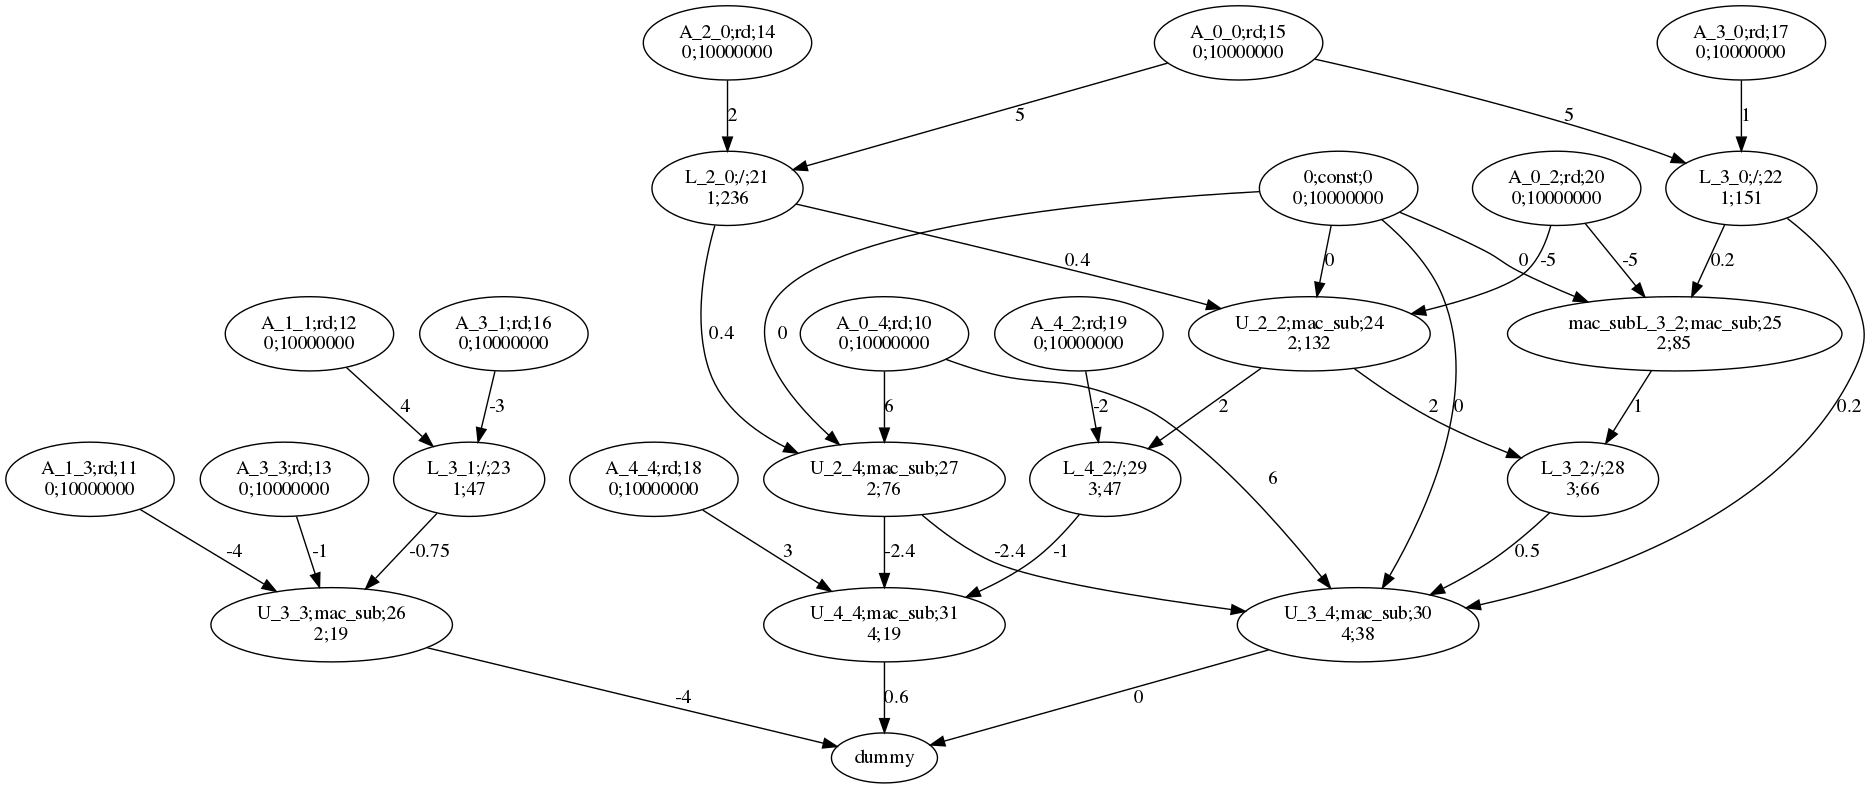
\includegraphics[width=7.5in,height=3.16043in]{./Scheduler/media/image44.png}
\begin{quote}
Fig 4.2.1(b): Data flow graph for computing LUD of matrix A mentioned in
section 3.1
\end{quote}

The meaning of terms inside each node of the data flow graph is described in the figure below: -

\begin{quote}
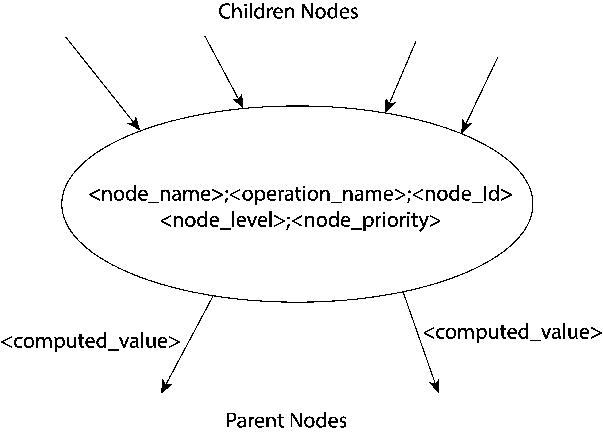
\includegraphics[width=2.70278in,height=1.9408in]{./Scheduler/media/image45.png}
Fig 4.2.1(c): A single node depicting the terms associated with the node
\end{quote}

The convention is used by children nodes and parent nodes in this
project. Nodes which are providing a value to a given node are \textbf{children} of the given node. And the nodes which are accepting values from a given node are \textbf{parents} to the given
node.

\textless node\_name\textgreater: Indicates the name associated with the node. The node name is of the form
\begin{quote}
``L\_x\_y'', ``U\_x\_y'', ``mac\_subL\_x\_y'' etc. The ``node\_name'' is
unique.

\textless operation\_name\textgreater: Indicates the operation performed by the node. The operations can be
\begin{quote}
``rd''(memory read), ``wr''(memory write), ``mac\_sub''(MAC), ``/''(DIV)
or
\end{quote}
\begin{quote}
``const''(indicates that the node has a constant value of 0).
\end{quote}


\textless node\_Id\textgreater: Indicates a unique Id associated with
each node.

\textless node\_level\textgreater: Indicates the level of the node i.e.
the worst-case distance from a leaf node.

\textless node\_priority\textgreater: It indicates the priority level of
the node. This parameter is handy while scheduling the graph.

\textless computed\_value\textgreater: This parameter indicates the
the value computed by the node.